\documentclass[10 pt,usenames,dvipsnames, oneside]{article}
\usepackage{../../../modelo-ensino-medio}


\begin{document}

\begin{center}
  \begin{minipage}[l]{3cm}

\includegraphics[width=2cm]{logo}    
\end{minipage}\hfill
\begin{minipage}[r]{.8\textwidth}
 {\Large \scshape Atividade: Analise de Infográficos}  
\end{minipage}
\end{center}
\vspace{.2cm}

\ifdefined\prof
\begin{objetivos}
\item \textbf{EM13MAT102} Analisar tabelas, gráficos e amostras de pesquisas estatísticas em relatórios divulgados por diferentes meios de comunicação, identificando, quando for o caso, inadequações que possam induzir a erros de interpretação, como escalas e amostras inapropriadas.

\item \textbf{EM13MAT406}: Construir e interpretar tabelas e gráficos de frequências com base em dados obtidos em pesquisas por amostras estatísticas, incluindo ou não o uso de softwares que interrelacionem estatística, geometria e álgebra.
\end{objetivos}


\begin{goals}
\begin{enumerate}
\item Análise de infográficos. Mais especificamente, analisar infográficos construídos pelo IBGE com os resultados da pesquisa PNAD/2015 referente ao suplemento especial de Prática de Atividades Físicas.

\item Explorar possíveis associações sobre a prática de atividades físicas com outras variáveis envolvidas na pesquisa, tais como sexo, nível de instrução e rendimento.
\end{enumerate}

\tcblower

\textit{\textbf{Infográfico 1}}

O item b) pretende estimular a reflexão sobre o papel da inferência estatística. De fato, foi observada uma amostra de domicílios de algumas cidades brasileiras, mas como a amostra foi cuidadosamente planejada e a estrutura da população brasileira é conhecida, foi possível dar um passo maior e calcular uma estimativa da proporção das pessoas de 15 anos ou mais que praticam atividades físicas no Brasil. A porcentagem $37{,}9$\%, realização numérica de um estimador, representa uma estimativa da proporção das pessoas de 15 anos ou mais que praticaram atividades físicas no Brasil (2015) (parâmetro). Observe que não foi realizado um censo para obter essa informação. Portanto, associada a essa estimativa existe uma margem de erro (valor correspondente à oscilação em torno da estimativa pontual) e um nível de confiança. Por exemplo, se o nível de confiança for $95$\% isso implica que para cada 100 amostras de mesmo tamanho, em $95$\% delas o parâmetro se situa no intervalo considerando a margem de erro. Claro que a margem de erro deve ser pequena e o nível de confiança alto na PNAD. Esses conceitos, margem de erro e nível de confiança, têm sido bem divulgados nas pesquisas eleitorais para o público em geral. Se for um ano de eleição, peça aos alunos para trazer resultados de pesquisas eleitorais incluindo a margem de erro e o nível de confiança. Cabe também destacar que todas as proporções apresentadas na pesquisa são estimativas que devem ter pequena margem de erro com nível de confiança alto. Assim, pequenas diferenças nessas proporções devem ser olhadas com cuidado, não sendo possível afirmar que elas são diferentes.

O item c) visa levar a uma reflexão sobre hábitos saudáveis. Por que achamos que a prática de atividades físicas é importante para a saúde de uma pessoa? Como essa conclusão foi obtida?

Os itens d) e e) têm como objetivo estudar possíveis associações entre duas variáveis qualitativas, a saber, sexo e prática de atividade física d) e faixa etária e prática de atividade física e). Observe que embora a idade seja uma variável quantitativa, quando ela é representada por faixas etárias ela se torna qualitativa.

É importante destacar, na análise desses gráficos, que o que se fez foi separar o conjunto de dados em subconjuntos como por exemplo, sexo feminino e sexo masculino e depois, observou-se a resposta sobre a prática de atividade física em cada subgrupo. Para efeito de comparação de grupos distintos, é importante trabalhar com a frequência relativa (ou porcentagem), pois os grupos podem ser de tamanhos diferentes e se os gráficos forem construídos com as frequências absolutas não será possível visualizar as relações entre as variáveis analisadas.

\textit{\textbf{Infográfico 2}}

Os itens f) e g) têm como objetivo estudar possíveis associações entre duas variáveis qualitativas, a saber, grau de instrução e prática de atividade física a) e rendimento per capita e prática de atividade física b). Observe que, embora rendimento seja uma variável quantitativa, quando ele é representado por intervalos de rendimento, se torna variável qualitativa. Novamente é importante destacar, nessa discussão, que o conjunto inteiro foi subdividido em subconjuntos ditados pelas categorias, grau de instrução ou faixas de rendimento, e que para cada subconjunto calculou-se a porcentagem de pessoas que praticam atividade física. Usar frequências absolutas não seria útil para comparar os diferentes grupos quando eles têm tamanhos diferentes.

\textit{\textbf{Infográfico 3}}


Na análise do infográfico 3, cabe destacar que trata-se de um gráfico de barras típico representando a distribuição de frequências de uma variável qualitativa. É importante levar os alunos a perceber que para a variável modalidade, considerando o conjunto de todas as pessoas que responderam essa questão, calculou-se as porcentagens para cada tipo de atividade indicada. Discuta sobre a categoria outras atividades indicando que foram respostas com frequência muito pequena e, de fato, não faria sentindo ir listando uma a uma essas modalidades. Em geral, nesses casos, o que se faz é agregar as respostas com frequência muito pequena na categoria outras. Sugira ao aluno pesquisar no link dessa pesquisa para verificar se, no instrumento de coleta de dados, essa questão era aberta (resposta livre) ou fechada (com opções a serem assinaladas).

Na análise desse gráfico, deve-se destacar que a altura das barras correspondem às porcentagens (frequências relativas) na qual ocorreram e que a soma dessas porcentagens será $100$\%. Também cabe comentar que as barras devem ter larguras iguais, mas não existe nenhum lugar geométrico definido ao longo do eixo horizontal para as respostas da variável modalidade de prática neste gráfico, ou seja, podemos mudar a posição das diferentes modalidades. As barras, separadas, são equidistantes e foram organizadas por ordem de decrescente de frequência. Como só há um eixo numérico (frequência), comente que as barras podem ser tanto verticais, como horizontais e essa orientação determinará a orientação do eixo que representa as frequências no gráfico.

\textit{\textbf{Infográfico 4}}

Na análise do infográfico 4, é importante destacar que foram usados dois tipos de gráficos diferentes para representar variáveis qualitativas, mas ambos usam a mesma ideia, a saber, uma região é subdividida de maneira harmônica em sub-regiões (o círculo em setores circulares e o retângulo em retângulos menores de mesma largura contidos nele) cujas áreas em relação à área da região correspondem exatamente à frequência relativa (ou porcentagem) da categoria de resposta que a sub-região representa. Por exemplo, a área do setor em vermelho dividida pela área do círculo é $0{,}147$ (ou $14{,}7$\% da área do círculo). A área do retângulo verde dividida pela área do retângulo inteiro é $0{,}578$ (ou $57{,}8$\% da área do retângulo inteiro). São duas formas de olhar como cada categoria de resposta aparece em relação ao todo.
\end{goals}

\bigskip
\begin{center}
{\large \scshape Atividade}
\end{center}
\fi

A seguir apresentaremos quatro infográficos (figuras \ref{est1-fig-2}, \ref{est1-fig-3}, \ref{est1-fig-4}, \ref{est1-fig-5}), produzidos pelo IBGE (\href{https://vamoscontar.ibge.gov.br/atividades/ensino-medio/9801-pesquisando-a-pratica-de-esportes-e-atividades-fisicas-no-brasil.html}{vamoscontar.ibge.gov.br}) usando os dados do Suplemento Prática de Esporte e Atividade Física da PNAD 2015.

Um \index{infográfico}infográfico é uma apresentação de informações integradas em textos sintéticos com dados numéricos e elementos gráficos e visuais tais como fotografias, desenhos, diagramas estatísticos, gráficos, etc.

\begin{figure}[H]
\centering


\noindent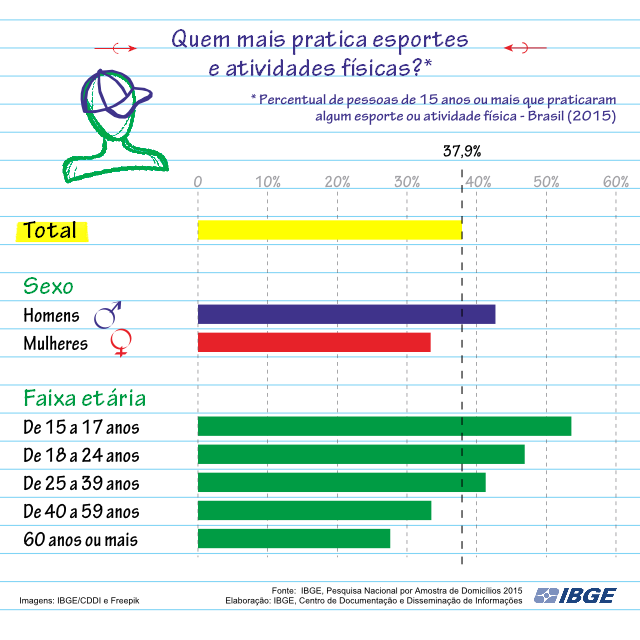
\includegraphics[width=250bp]{PNAD_2015_Esportes_01quem2.png}
\caption{PNAD - Infográfico 1}
\label{est1-fig-2}
\end{figure}

\begin{figure}[H]
\centering


\noindent\includegraphics[width=250bp]{{PNAD_2015_Esportes_03instrrend2}.png}
\caption{PNAD - Infográfico 2}
\label{est1-fig-3}
\end{figure}

\begin{figure}[H]
\centering

\includegraphics[width=250bp]{{PNAD_2015_Esportes_04principais}.png}
\caption{PNAD - Infográfico 3}
\label{est1-fig-4}
\end{figure}

\begin{figure}[H]
\centering


\noindent\includegraphics[width=250bp]{{PNAD_2015_Esportes_05investimento}.png}
\caption{PNAD - Infográfico 4}
\label{est1-fig-5}
\end{figure}

\begin{enumerate}
\item {} 
Segundo os resultados da pesquisa (veja a \hyperref[est1-fig-2]{figura \ref{est1-fig-2}}), qual a porcentagem de pessoas de 15 anos ou mais que praticaram algum esporte ou atividade física no período de um ano?

\item {} 
O título genérico do infográfico da \hyperref[est1-fig-2]{figura \ref{est1-fig-2}}, a saber, “Quem mais pratica esportes e atividades físicas? - Percentual de pessoas de 15 anos ou mais que praticaram algum esporte ou atividade física-Brasil (2015)”, diz respeito à população brasileira de 15 anos ou mais ou à amostra coletada?

\item {} 
Com base nas recomendações médicas sobre a prática de atividades físicas para se ter boa saúde, como você avalia o resultado obtido na pesquisa para a população brasileira de 15 anos ou mais?

\item {} 
Considerando homens e mulheres separadamente, percebe-se alguma diferença com relação à prática de atividades físicas? Em caso afirmativo, descreva a(s) diferença(s) observada(s).

\item {} 
Considerando as faixas etárias discriminadas no infográfico, percebe-se alguma diferença com relação à prática de atividades físicas? Em caso afirmativo, descreva a(s) diferença(s) observada(s).

\item {} 
Considerando os diferentes graus de instrução (\hyperref[est1-fig-3]{figura \ref{est1-fig-3}}), percebe-se alguma diferença com relação à prática de atividades físicas? Em caso afirmativo, descreva a(s) diferença(s) observada(s).

\item {} 
Considerando as faixas de rendimento mensal per capita do domicílio, percebe-se alguma diferença com relação à prática de atividades físicas? Em caso afirmativo, descreva a(s) diferença(s) observada(s).

\item {} 
Qual foi a variável estudada no gráfico da \hyperref[est1-fig-4]{figura \ref{est1-fig-4}}?

\item {} 
A variável estudada no gráfico da \hyperref[est1-fig-4]{figura \ref{est1-fig-4}} tem respostas de que tipo: numéricas ou não-numéricas?

\item {} 
Qual foi a resposta que apresentou a maior frequência no gráfico da \hyperref[est1-fig-4]{figura \ref{est1-fig-4}}?

\item {} 
O que você acha que representa a resposta “Outros Esportes” no gráfico da \hyperref[est1-fig-4]{figura \ref{est1-fig-4}}?

\item {} 
Qual a porcentagem de pessoas de 15 anos ou mais que concorda com que o poder público deva investir em atividades físicas ou desportivas (\hyperref[est1-fig-5]{figura \ref{est1-fig-5}})?

\item {} 
Qual a opinião das pessoas de 15 anos ou mais que concordam que o poder público deve investir em atividades físicas ou esportivas com relação à prioridade de investimentos?

\item {} 
Entre as pessoas de 15 anos ou mais que não concordam que o poder público deve investir em atividades físicas ou esportivas, que área elas entendem como prioritária?

\item {} 
Podemos afirmar que 57,8\% das pessoas de 15 anos ou mais defendem que o poder público deve investir em Saúde?"

\end{enumerate}

\ifdefined\prof
\begin{solucao}
\begin{enumerate}

\item $37{,}9\%$

\item População brasileira de 15 anos ou mais.

\item Não parece satisfatório. Vários estudos têm demonstrado que a prática de atividades físicas é fundamental para se ter boa saúde.

\item Sim. Entre os homens brasileiros de 15 anos ou mais, pouco mais de $40$ praticam atividade física; enquanto esse percentual para mulheres brasileiras de 15 anos ou mais é pouco menor do que $35\%.$

\item Sim. Percebe-se uma diminuição dos percentuais de pessoas que praticam atividade física, conforme a idade aumenta. Na faixa de 15 a 17 anos temos mais de $50\%$, na faixa de 18 a 24 anos temos um pouco menos do que $50\%$ na faixa de 25 a 39 anos temos pouco mais de $40\%$, na faixa de 40 a 59 anos temos mais de $30\%$ e na faixa 60 anos ou mais temos menos de $30\%$.

\item Sim, a porcentagem de pessoas de 15 anos ou mais que pratica atividade física cresce conforme o grau de instrução é maior.

\item Sim, a porcentagem de pessoas de 15 anos ou mais que pratica atividade física cresce conforme a faixa de rendimento per capita é maior.

\item Modalidade de atividade física praticada.

\item Não-numéricas: futebol, natação, etc.

\item Futebol

\item Como as últimas modalidades discriminadas no gráfico apresentaram porcentagens muito pequenas (“ciclismo”, “ginástica rítmica e artística”, “lutas e artes marciais”, “voleibol, basquetebol e handebol”), cerca de $2\%$, a categoria outros esportes reuniu modalidades que ocorreram com porcentagens muito pequenas, não cabendo representá-las separadamente no gráfico. Observe que a última modalidade, antes de “outros esportes” já está reunida em mais de uma modalidade, a saber, “voleibol, basquetebol e handebol”.

\item $73,3$\%

\item Entre as pessoas que acham que se deva priorizar investimentos em atividades físicas, $91{,}1\%$ acha que o investimento deve ser para atividades físicas para as pessoas em geral, $8\%$ acha que deve ser para a formação de atletas e, o restante ($0{,}9\%$) respondeu outro tipo de prioridade.

\item Entre as pessoas que não concordam que o poder público deve investir em atividades físicas, $57{,}8$\% acham que a prioridade deve ser Saúde, $21{,}3\%$ acham que a prioridade deve ser Segurança, $16{,}5\%$, acham que a prioridade deve ser Educação e, o restante ($4{,}4\%$) respondeu outros tipos de prioridade.

\item Não, de fato, são $57{,}8\%$ de $14{,}7\%$ o que dá cerca de ${,},5\%$ das pessoas de 15 anos ou mais.

\end{enumerate}
\end{solucao}
\fi

\end{document}